\documentclass{article}




\title{Bayesian Analysis of Randomized Controlled Trials}
\author{Julian Bautista$^\dag$, Alex Pavlakis$^\dag$, Advait Rajagopal$^\dag$}
\providecommand{\keywords}[1]{\textbf{Keywords --} #1}
\date{\today}
\setlength{\parskip}{1.2ex} % show new paragraphs with a space between lines
\setlength{\parindent}{0em} % get rid of indentation for new paragraph

\usepackage{amsmath}
\usepackage{latexsym}
\usepackage{graphicx}
\usepackage{amsfonts}
\usepackage{wasysym}
\usepackage{amssymb}
\usepackage{mathrsfs}
\usepackage{multirow,array}
\usepackage{booktabs}
\usepackage{float}
\usepackage{color}
%
\usepackage[margin=1.1811in,bottom=1in,top=1.1811in]{geometry}
\usepackage{fancyhdr}
\pagestyle{fancy}
\usepackage{blindtext}

\lhead{}
\chead{Bautista, Pavlakis, Rajagopal}
\rhead{}
%\lfoot{\textit{STATGR6103 Final Project}}
\cfoot{}
\rfoot{\thepage}
\renewcommand{\headrulewidth}{1pt}
%\renewcommand{\footrulewidth}{1pt}
%
\DeclareMathAlphabet{\mathpzc}{OT1}{pzc}{m}{it}
\linespread{1.8}
\usepackage{listings}
\usepackage[most]{tcolorbox}
\usepackage{inconsolata}
\newtcblisting[auto counter]{sexylisting}[2][]{sharp corners, 
    fonttitle=\bfseries, colframe=black, listing only, 
    listing options={basicstyle=\ttfamily,language=java}, 
    title=Listing \thetcbcounter: #2, #1}
    \newcommand\blfootnote[1]{%
  \begingroup
  \renewcommand\thefootnote{}\footnote{#1}%
  \addtocounter{footnote}{-1}%
  \endgroup
}
%%%%%%%%%%%%
%   Document starts   %
%%%%%%%%%%%%

			
\begin{document}
\maketitle
\blfootnote{$\dag$The New School for Social Research, 6 E 16 St, New York, NY, 10003.}
\iffalse

\abstract{Bayesian Data Analysis is a powerful tool for incorporating data and prior information into complex and flexible models.  It is well-suited to analyze Randomized Control Trials, where effects are small and data has hierarchical structures.  In this paper, we summarize the approach and methods of Bayesian Data Analysis, and demonstrate how they can be applied to a Randomized Control Trial measuring the effect of a smartphone application on binge eating behavior.  We fit a hierarchical Poisson model, which accounts for individual level and time level effects, allowing us to model treatment effects over time.  Our analysis suggests that the smartphone application may cause a small reduction in the number of Objective Bulimic Episodes in some stages.  Bayesian methods allow us to account for the structure of the data, obtain heterogenous treatment effects for different stages of the therapy, and incorporate uncertainty in our parameter estimates. We conclude that Bayesian methods have the potential to improve analyses of Randomized Control Trials in many fields.}	
\fi

\newpage

\section{Introduction [Rewrite]}
Bayesian methods are gaining popularity because they allow researchers to incorporate all available information into flexible and transparent statistical models.  Many researchers have begun to incorporate Bayesian methods into medical, pharmaceutical, and social-science research.  The purpose of this paper is to show how Bayesian methods can be the standard in applied research.  We provide a general overview of the approach and an example analysis of Randomized Control Trial (RCT) on the impact of a smartphone application on eating disorder behavior. 
Regression models are well-suited for analyzing RCTs because they allow researchers to estimate causal effects more precisely by controlling for all available pre-treatment covariates [Gelman and Hill, 2007].  The Bayesian approach to regression models is advantageous because it allows researchers to include relevant prior information, to fit flexible models, and to naturally estimate varying treatment effects among subgroups of the population.

Randomized controlled trials (RCTs) designed to test the efficacy of treatments for binge eating and/or purging for binge eating disorder (BED), bulimia nervosa (BN), or subthreshold variants are an essential methodological tool for clinical researchers in the field of psychiatry.  The primary outcomes of these RCTs are often symptom counts (e.g., objective or subjective binge episodes, vomiting, laxative use, etc.). This data is typically positively skewed and often include inflation of zeros representing achievement of abstinence or symptom remission.  Grotzinger, Hildebrandt, and Yu [2016] discuss these issues and their implications for analyzing RCTs.  Specifically, they use simulated data to examine the value of several different models of positively skewed data, including latent growth zero inflated Poisson (ZIP), zero inflated negative binomial (ZINB), and semi-continuous models.  Their results suggest that semi-continuous models have some desirable analytic properties, including greater statistical power in most situations over traditional continuous models.  In this paper, we present a robust alternative to these latent growth models in the form of Bayesian hierarchical model.  We aim for this paper to be an introduction to the method with a focus on providing guidelines for executing this method in a rigorous way and with enough information to facilitate replication of these methods.  To achieve this goal, we use the data from recently published RCT examining the efficacy of cognitive behavioral therapy version of guided self-help (CBT-GSH) with the addition of a smartphone app designed for the intervention [Hildebrandt et al., 2017]. 

The main contribution of this paper is a demonstration of Bayesian methods. We believe these methods are rigorous, reproducible, and open to checking. Bayesian analysis makes modeling assumptions explicit with the use of prior distributions of underlying parameter values which consider all  problems for which the model could apply.  The rest of the paper is organized as follows, section 2 explains the process and steps of Bayesian data analysis and inference. Section 3 compares Bayesian analysis to other methods, section 4 explains the experiment, modeling and results. Section 5 concludes and section 6 has the Stan code used for this model.

\section{Bayesian Data Analysis}
Bayesian data analysis (BDA) is a method of building statistical models to describe data.  Researchers begin with explicit assumptions about the data generating process based on past research and the scientific nature of the problem. They then design experiments or observational studies based on these beliefs and assumptions to collect data. Using Bayes' rule they combine their assumptions or \textit{prior} information with the actual data into a comprehensive probability model. This model contains information about all known (observed data) and unknown (unobserved parameters) quantities related to the data generating process.
There are three main steps to BDA which are listed below and explained in detail in the subsequent sections:
\begin{enumerate}
\item Specify a model based on scientific knowledge of the data generating process at hand.
\item Estimate model parameters based on observed data.
\item Evaluate the model's accuracy and expand or alter the model as needed.
\end{enumerate}

\subsection{Probability notation and Bayes' rule}
In Bayesian Data Analysis, assumptions are specified mathematically as \textit{prior distributions}.  Data is represented through a \textit{likelihood model}. Bayes' Rule combines prior distribution and data likelihood into a \textit{posterior distribution}.  A formal expression of the Bayes' Rule is as follows;
\begin{align}
{p(\theta| y, x) = \frac{ p(\theta) p(y|\theta, x)}{p(y)}}
\end{align}
$\theta$ is the estimated parameter. In the context of an RCT, $\theta$ is the effect of the treatment $x$ on dependent variable $y$. $p(\theta)$ is the prior distribution of the treatment effect, which captures the researcher's beliefs about the model parameter prior to any analysis. $p(y | \theta, x)$ is the likelihood function and is the probability of the observed data given the parameter.  $p(y)$ is a normalizing constant with respect to $\theta$ that ensures the left hand side $p(\theta |y, x)$ is a proper probability distribution that integrates to 1. For a full treatment of proper distributions and normalizing constants see Gelman et. al [2013]. \\
For our purpose, we can ignore this denominator and rewrite the expression for the posterior $p(\theta | y)$ (equation 1) as ;
 \begin{align}
 p(\theta | y, x) \propto p(\theta) p(y |\theta, x)
 \end{align}
The posterior distribution is proportional to the product of the prior and the likelihood. Ultimately the goal of our modeling exercise is to learn the posterior distribution $p(\theta|y, x)$ and summarize it accurately [Gelman et. al. 2013]. Based on this we can make inferences and predictions.

\subsection{Model development}
Model development involves setting up a joint probability distribution that accounts for all observed data and unobserved parameters. The model should include all knowledge of the experiment or data collection process and should be logically consistent with scientific nature of the problem at hand. We approach model development in three steps.

\subsubsection{Exploratory data analysis}
Summarizing the initial results from data through visualizations and summary statistics is a critical model building step. We look at summary statistics of our relevant variables to understand their distribution. We explore the data through univariate analyses, such as histograms to visualize distributions, and bivariate analyses, such as scatter plots of potential dependent and independent variables against each other to see if there are meaningful linear or non linear relationships. This exploratory process informs us of the distribution of individual variables, their correlations, and other relevant information for modeling. \\
Exploratory analysis helps us to choose an appropriate likelihood model to describe the data. For example, if our variables are normally distributed and linearly correlated, we might choose a simple linear regression model. If the relationship between variables is not so straightforward we might choose more complicated models.  It allows the researcher to explore and solidify intuition about the problem at hand and the nature of the data. An introductory treatment of exploratory data analysis can be found in Tukey [1977]. A more advanced explanation of exploratory data analysis, particularly in the context of Bayesian statistics, is available in Gabry et. al [2018] and Betancourt [2018].


\subsubsection{Setting up a likelihood model}
The likelihood function will be familiar to non-Bayesians, as it is often analogous to a traditional regression equation. Like traditional regression, the researcher must select the appropriate independent variables that represent important determinants of the outcome variable. The regression model represents the probability of the outcome variable given the independent variables and model parameters. To choose the right likelihood function, it is critical to know the type of data. Data can be binary, categorical, ordinal, count, or continuous and each of these types of data requires a different kind of model.  For example, if the outcome variable is binary (0 or 1), a logistic regression framework may be appropriate. If data is continuous and defined on the entire real line, a normal regression will fit better. In this paper we deal with Objective Binge Eating (OBE) episodes as the outcome variable. These are non-negative and discrete in nature so we choose a Poisson likelihood function (see section 4.2). 
 
\subsubsection{Choosing a prior distribution}
The prior distribution is a mathematical encoding of the researcher's starting assumptions. A prior distribution serves three functions. First, it regularizes or constrains the parameter space by specifying likely ranges for parameter values. Second, it makes assumptions about the underlying scientific nature of the problem explicit. Third, it facilitates the calculation of a posterior distribution and makes it possible to have posterior simulations or ``draws" from the posterior. \\
Prior choice depends on the parameter or coefficient of interest.  We could assign a completely ``noninformative" or flat prior to our coefficient by specifying a uniform distribution as the prior. This is equivalent to saying that our parameter is equally likely to assume any value from negative infinity to positive infinity and we have no more information about it. Using a noninformative uniform prior is the same as carrying out a maximum likelihood estimation of the parameter of interest. \\
It is hardly ever true that researchers know nothing about the problem at hand or relevant parameters. They often possess valuable information about the parameter and statisticians can use ``weakly informative" or ``specific informative priors" to reflect the researchers' knowledge. For instance, if a coefficient of interest is a percentage, then it \emph{must} be between 0 and 1, and we can assign a \emph{Beta} prior distribution to that coefficient.  If we believe that a coefficient is close to zero, but may be positive or negative, we could assign a more informative \emph{Normal}(0, 1) prior distribution to it.  More information about prior choice and considerations for the same can be found on the GitHub page for Stan developers [Stan Developers, 2013]. We explain the Bayesian probabilistic programming language, Stan, in section 2.3.\\


\subsection{Model estimation}
Once the likeilihood model and prior distribution are specified, the posterior distribution of our outcome variable can be estimated. As discussed in section 2.1, the posterior distribution is obtained by simply multiplying the prior and likelihood functions. The distribution obtained by this process is proportional to the true posterior because we generally tend to ignore the normalizing constant (the denominator in equation 1). We use an approximation of the posterior as shown in equation 2 because calculating the true posterior analytically may be practically impossible.  A standard practice is to use Markov Chain Monte Carlo (MCMC) sampling methods to approximate the posterior up to a normalizing constant and sample from it. There are  other approaches to calculating the posterior distribution, but those are beyond the scope of this paper. Analyses in this paper are carried out with the Bayesian probabilistic modeling language Stan \textbf{[SOURCES TO UNDERSTAND STAN]}. Stan uses a Hamiltonian Monte Carlo sampling algorithm (from a broader class of MCMC sampling methods) to approximate the posterior distribution. Betancourt [2017] has a clear exposition of how the algorithm works. Stan returns to us the posterior distribution of the desired parameters. Stan can also predict values based on the specified model. These predictions are basically random draws from the posterior distribution and can be used for model checking, validation, and expansion.

\subsection{Model checking, comparison and expansion}
It is essential to evaluate our statistical analysis with model checking. We begin by evaluating the performance of our model by ensuring that it converges on robust parameter estimates and that the results make sense given what we know about the observed data and the problem itself. We also need to check how sensitive our results are to the modeling assumptions and the priors. Sometimes using stronger priors can help with convergence and more stable results. We use the posterior distributions of the parameters to check our model by carrying out \textit{posterior predictive checks}. These could be graphical checks where we simulate ``fake" data from our model and compare it graphically to the original data. We could also use certain test statistics (eg. mean, minimum value etc.) and compare the values of those statistics across models and see how close they are to the ground truth obtained from the observed data itself.\\
Based on the fit of the model, we can engage in model comparison. We are not explicitly looking to choose the ``right" model because there is no truly perfect model that can recover the data generating process. We iteratively build better models by including or excluding parameters or predictors. Then we engage in a key step called model comparison. We check the robustness of parameters across models as well as compare posterior predictive performance. It is up to the researcher to choose which model best fits the problem, but in the interest of replicability it is always good to make all assumptions, models, and data accessible and public. This leaves the study open to future research, scientific critique and model expansion. The way we obtain our priors from knowledge of the problem and experts in the field, other researchers may want to derive their priors for future experiments and analyses from this study.\\
\textbf{[add more model checking techniques!]}

\section{Advantages of BDA}
In this section we discuss some of the major benefits of using a Bayesian approach to the analysis of Randomized Control Trials.

\subsection{Heterogenous Treatment Effects}
Perhaps the greatest advantage of Bayesian modeling is its ability to capture heterogeneity in the sample and provide treatment effects that account for this heterogeneity. For example in our study, we control for variation in demographic variables and, importantly, variation in the treatment across the time . This type of approach is commonly known as a varying slope - varying intercept model [Gelman and Hill, 2007]. Our approach of hierarchical modeling and partial pooling allows us to accomplish this naturally, which is among of the greatest advantages of BDA as a method. \\
Hierarchical (multilevel) modeling has two closely related meanings [Feller and Gelman, 2015]. Hierarchies can explain a hierarchical data structure like spatial or temporal variation. In the RCT we consider in this paper, each treatment period is treated as a level and so we obtain different treatment effects for each period. Hierarchies also describe how parameters are modeled. We model our treatment effects for each level or category in the data, to come from a common underlying prior distribution \textbf{[ ADD CITATION HERE]}. This is the idea of \textit{partially pooled} estimates of treatment effects. Partial pooling in a Bayesian context is different than traditional complete pooling or no pooling approaches. \\

In a non-Bayesian method, there are two choices a researcher has: a complete pooling model, and a no pooling model. With complete pooling, the categories in data are completely interchangeable, thus ignoring the uniqueness of categories. With no pooling, each category is treated as independent of the others, thus ignoring the interrelatedness of each of the categories.  For example, if an RCT was conducted in multiple locations by different staff, the researcher must assume that the treatments are entirely identical in a complete pooling model, ignoring the differences in execution that may have taken place by differing staff. In the no pooling model, the RCT would assume that each treatment would be entirely different across locations, despite having close similarities in how the treatments were applied. Setting up a prior distribution allows researchers to solve this problem by saying that the treatment effects across the locations have a common mean, but vary based on location. Thus partial pooling is often more accurate as it takes into account both the uniqueness and interrelatedness of categories within a hierarchical model. \textbf{[Consider improving/rewriting no pooling, partial pooling and complete pooling]}, \textbf{Explain hyperparameters before using the term in Section 4 equation 6, perhaps in the context of partial pooling]}



\subsection{Making uncertainty explicit}
Bayesian Data Analysis has fundamentally different assumptions compared to frequentist approaches. For starters, BDA assumes a generative probability model. The classical frequentist paradigm states that if an experiment were to be repeated infinite times, estimates would fall within the 95\% interval with a probability of 0.95. In this way, frequentist results rely heavily on asymptotics. Error in the models represent sampling error associated with a test statistic, not genuine uncertainty. Meanwhile, Bayesians start out with a prediction of the parameters to be estimated based on certain assumptions encapsulated in the prior and iteratively update these estimates mathematically using the new information contained in the data. This is a superior estimate because it does not constrain the estimates to move asymptotically towards a specific, pre-defined distribution. Instead, it allows the assumptions and data to meet together to form a distribution that captures the uniqueness of the specific scientific problem. This is often a more accurate representation of uncertainty.\\
Furthermore, models that use priors have access to information beyond what was collected within the study. Data does not live only on the spreadsheet. It is contained in the researcher's knowledge of the literature, the data generating process, and the specific scientific problem. This can include common sense knowledge such as the understanding that estimates on ratios will be between 0 and 1, or it could be an expected estimate based on previous studies done. Regardless of the source of the information, knowledge about an estimator can be translated into the prior to improve accuracy. \\ 
By embracing the uncertainty inherent in statistical estimators, the Bayesian approach leaves little need for the p-values that are often used as thresholds in classical statistics.  Intuitively, p-values represent the probability of the data conditional on the null hypothesis, under hypothetical replications.  However, since researchers have many opportunities to choose how data is coded, which data is included, and what comparisons are made, it is easy to obtain ``statistically significant" p-values even if there are no ``true" effects [Gelman, 2017].  In the Bayesian approach, we focus on the posterior distribution of parameters, leaving no need for worrying about hypothetical replications or the issue of multiple comparisons.



\subsection{Transparency}
Bayesian analysis also lends itself to better scientific scrutiny on models overall. This occurs because non-Bayesian techniques and traditional frequentist models make tacit assumptions. Bayesian methods make underlying modeling assumptions explicit in the form of a prior. [\textbf{For example, a simple linear regression tacitly assumes that the parameter is normally distributed and has a uniform prior. - rewrite?}] While this assumption may be appropriate for some problems, in many occasions it does not get scrutinized closely because it is an implied assumption. Meanwhile, the power of a prior to influence estimates puts a magnifying glass on model selection issues that are easily glossed over in frequentist methods.  Close scrutiny is a critical component for rich academic discourse. It puts the onus on researchers to justify the assumptions of their model and allows for vibrant discussion. Abandoning a p-value based, binary ``reject" or ``fail to reject" approach allows us to engage in iterative model building and compare across models. Making our modeling approaches and statistical analysis public to facilitate comparison and constant improvement enables us to be more transparent at all steps of the analysis.

\section{Impact of Smartphone App on Eating Behavior}

Hildebrandt et. al [2017] conducted an experiment to test whether the Noom Monitor, a smartphone application, could augment the effect of in-person therapeutic treatment on binge eating behavior.  The treatment, known as \emph{guided self-help treatments based on cognitive-behavior therapy} (CBT-GSH), had been shown in previous research to reduce binge eating behavior by 10-50\%.  The Noom Monitor application was designed to facilitate CBT-GSH.  For this example, we consider two research questions from the experiment:
\begin{enumerate}
\item{Is CBT-GSH more effective at reducing binge eating behavior when facilitated by the Noom Monitor?}
\item{Does the effect of the Noom Monitor vary over time?}
\end{enumerate}

\subsection{Experimental design}

66 men and women with Bulimia Nervosa (BN) or Binge Eating Disorder (BED) were randomly assigned into two treatment conditions: CBT-GSH (N= 33) or CBT-GSH + Noom (N=33).  Therapy lasted for 12 weeks.  Assessments were conducted at weeks 0, 4, 8, 12, 24, and 36.  The primary outcome was Objective Bulimic Episodes (OBE).  

\subsection{Model development}
\subsection*{Exploratory data analysis}
Figure 1 displays OBEs per week for each individual in both treatment conditions.  A few aspects of the data immediately stand out, which suggest that any model should account for individual-level effects and time-level effects, and should let treatment effects vary over time.  
\begin{itemize}
\item{The number of OBEs decreases over the course of the treatment for almost all subjects.}
\item{The biggest decreases in OBEs appear to occur in the early stages of treatment.}
\item{The primary sources of variation in OBE appear to be \emph{between people} and \emph{over time}.}
\end{itemize}
%
\begin{figure}[H]
   \begin{center}
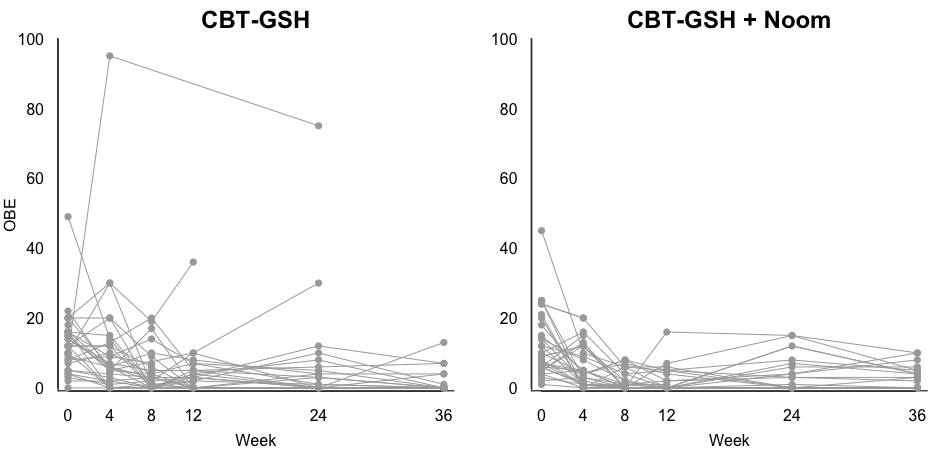
\includegraphics[width=\textwidth, height=\textheight, keepaspectratio]{Noom_paths.png}
   \end{center}
\caption{\emph{Fig.1 (a) and (b) show the OBE measurements for individuals in the CBT-GSH group and CBT-GSH + Noom group respectively. The horizontal axis shows the week and the vertical axis shows the instances of OBE. The gray dots represent OBE readings over time for each individual. }}
\end{figure}
%
Figure 2 displays the distribution of OBEs in each condition in each week.  We notice three characteristics of the data from these histograms.
\begin{enumerate}
\item{The distributions appear to condense around zero for both conditions over time} 
\item{The distributions in the CBT-GSH condition appear to have longer tails than those in the CBT-GSH+Noom condition}
\item{OBEs are count data; they must be nonnegative integers.}
\end{enumerate}
These three characteristics suggest that the appropriate model for OBEs is the Poisson distribution, because it is restricted to nonnegative integers and can concentrate its density around low numbers with a long tail.
%
\begin{figure}[H]
\begin{center}
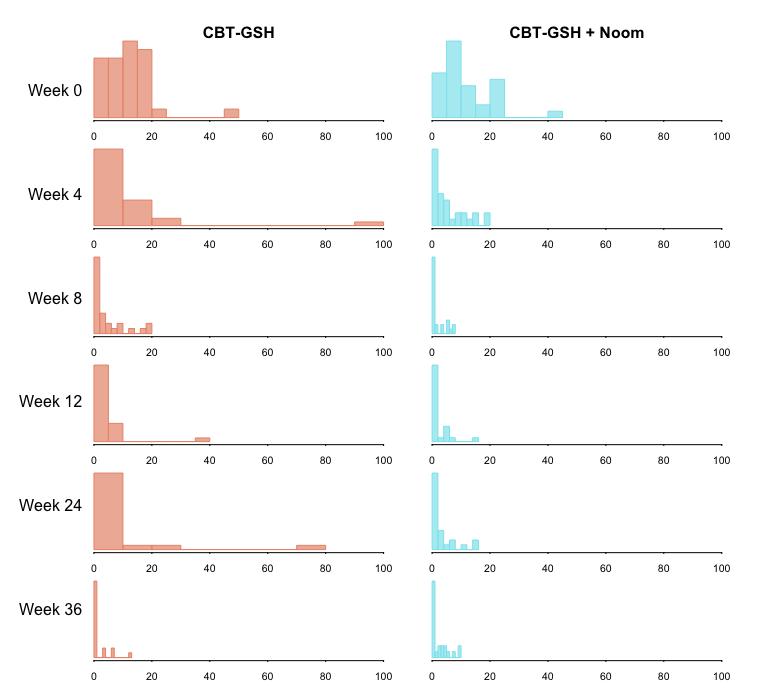
\includegraphics[width=\textwidth, height=\textheight, keepaspectratio]{noom_hist.png}
\end{center}
\caption{\emph{Histograms display the distribution of OBEs in each condition in each stage of the treatment. The orange and light blue histograms show the distribution of OBEs for the CBT-GSH and CBT-GSH  + Noom group respectively.}}
\end{figure}
%
\subsection*{Setting up a likelihood}

We analyze RCTs by modeling the outcome of interest (in this case OBE) as a function of the treatment and all available pre-treatment covariates.  The coefficients associated with the treatment are estimates of average treatment effects.  Inclusion of all available pre-treatment covariates accounts for variation in the outcome variable, decreasing uncertainly around treatment effects and providing the model with more predictive power.  We conduct \emph{intent-to-treat} analysis, meaning that our inferences will be based on initial treatment assignment, and will not account for mid-experiment dropouts. \\
The outcome variable is restricted to be nonnegative integers, so we fit a Poisson regression model, with hierarchies on individuals, time periods, and treatment effects. [expound here and compare to ZIP] For each individual in each time period, the number of OBEs follows a Poisson distribution, with a mean dependent on the characteristics of the individual and the time period.  
\begin{align}
OBE_{i,t} &\sim Poisson(\lambda_{i,t}) \\
\lambda_{i,t} &= exp(\alpha_i + \beta_t + \gamma_tT_i + X_i\theta) \\
T_i &=
    \begin{cases}
      0, & \text{if}\ CBT-GSH \\
      1, & \text{if}\ CBT-GSH + Noom \\
    \end{cases}
\end{align}
$\alpha$ is an individual-specific intercept, $\beta$ is a time-specific intercept, $\gamma$ is a time-specific treatment effect, $T$ is a treatment indicator, $X$ is a matrix of individual level covariates (age, sex, race, etc), and $\theta$ is a vector of effects. Subscripts $i = 1, ..., 66$ indicate individuals and subscripts $t = 0, 4, 8, 12, 24, 36$ indicate time periods.

\subsection*{Choosing a prior distribution}
Table 1 has a list of different sources from which prior information has been obtained for this experiment. It aims to summarize the various methods which a researcher can use to incorporate prior information into the modeling process. There is a rich literature on binge-eating disorders and bulimia nervosa studies, implying a large amount of prior information. This makes analysis of similar RCTs amenable to Bayesian methods. For more examples of priors see the Appendix.
%
\begin{table}[H]
\centering
\begin{tabular}{r l}
  Source of Prior Information &  \\ 
  \hline  \vspace{0.25em}
  Experimental Design & Outcome variable is nonnegative integers \\
  \vspace{0.25em}
  Literature & Treatment effect size is small \\
                  & A large number of zeros in OBE data due to remission\\
  Exploratory Data Analysis & There is variation in OBEs at the individual level \\
					  & There is variation in OBEs over time \\
                                            & Treatment effects may vary over time \\
    \hline
\end{tabular}
\caption{\emph{Sources of prior information.}}
\end{table}
%
We believe that individual-level intercepts are simultaneously unique to the individual and common to the population; that is, each individual has their own baseline predilection to engage in eating disorder behavior, but those baseline predilections are not drastically different from each other.  We operationalize this concept by modeling all individual-level intercepts as coming from a common distribution, with \emph{hyperparameters} $\mu_{\alpha}$ and $\tau_{\alpha}$.  In Bayesian statistics, hyperparameters are parameters of prior distributions.  In hierarchical models, we model hyperparameters explicitly.
%
\begin{align}
\alpha_i \sim Normal(\mu_{\alpha}, \tau_{\alpha}) \ \forall \ i \in 1,...,66
\end{align} 
%
Similarly, we believe that time-specific treatment effects may be unique to each period but similar over time. We operationalize this concept by modeling all time-specific treatment effects $\gamma$ as coming from a common distribution, with \emph{hyperparameters} $\mu_{\gamma}$ and $\tau_{\gamma}$.
%
\begin{align}
\gamma_t \sim Normal(\mu_{\gamma}, \tau_{\gamma}) \ \forall \ t \in 0, 4, 8, 12, 24, 36
\end{align} 
%
$\mu_{\gamma}$ is the \emph{grand mean}, the overall treatment effect; $\tau_{\gamma}$ is the variation in treatment effects over time; and each individual $\gamma_t$ is a time-period specific treatment effect.  This approach has a natural smoothing effect: any extreme estimates of $\gamma_t$ will be partially-pooled back toward the grand mean $\mu_{\gamma}$.\\
%
We assign the following prior and hyperprior distributions:
\begin{align}
\mu_{\alpha} &\sim Normal(5, 5) \\
\tau_{\alpha} &\sim Cauchy^+(0, 30) \\
\mu_{\gamma} &\sim Normal(0, 5) \\
\tau_{\gamma} &\sim Cauchy^+(0, 30) \\
\theta &\sim Normal(0, 1)
\end{align}
%
The normal distributions around the individual and treatment effects allow us to guide the model to the appropriate range of parameter values, but with wide enough variance (5 in each case) to let the model find its own way in that range.  Half cauchy priors on the variance parameters are weakly informative, with much of their mass around zero but gentle slopes in their tails, which have been shown to be effective prior distributions for variance parameters [Gelman, 2006].

\subsection{Model estimation and results}
We estimate this model with \emph{Hamilton Monte-Carlo} in Stan.  Model code is appended to this document. This is a particular algorithm from a larger class of Markov Chain Monte Carlo algorithms, for more examples see Gelman et. al [2013].

Model results are displayed in Table 2.  Results suggest that using the Noom Monitor smartphone application during CBT-GSH may slightly decrease OBEs.  There is evidence that the treatment effect varies over time, with the Noom effect being slightly more pronounced during stages 4, 8, 12 and 24 of therapy but decreasing by week 36.\\

\begin{table}[H]
\centering
\begin{tabular}{r c c c c c}
  \hline
 & mean & 25\% & 50\% & 75\%\\ 
  \hline
  $\gamma_0$ & 0.18 & -0.45 & 0.15 & 0.78  \\ 
  $\gamma_4$ & -0.43 & -1.05 & -0.46 & 0.16 \\ 
  $\gamma_8$ & -0.70 & -1.33 & -0.71 & -0.10 \\  
  $\gamma_{12}$ & -0.65 & -1.28 & -0.68 & -0.04 \\  
  $\gamma_{24}$ & -0.72 & -1.34 & -0.75 & -0.11 \\  
  $\gamma_{36}$ & 0.21 & -0.42 & 0.19 & 0.82 \\ 
  \hline \hline
  $\mu_{\gamma}$ & -0.34 & -0.98 & -0.36 & 0.26 \\ 
  $\tau_{\gamma}$ & 0.64 & 0.43 & 0.56 & 0.77 \\ 
   \hline
\end{tabular}
\caption{\emph{Table displays model results for Noom effects in all six time periods and grand mean and variance parameters.}}
\end{table}


\subsection{Model checking, comparison, and expansion}
Before using our model to make inferences about time-specific treatment effects, we check its fit by comparing model-simulated OBE to data OBE.  If model simulations do not track the data well, we may want to revisit our model's assumptions before trusting its inferences.  If the model's simulations recover patterns in the data, we are more inclined to trust it. \\
Figure 3 displays OBEs in each period for each individual in each treatment group, from raw data (upper plots) and model simulations (lowers plots).  Black lines display means for each period.  This suggests that the model is able to pick up on the key variables that determine OBE over time for the duration of this experiment.
%
\begin{figure}[H]
\begin{center}
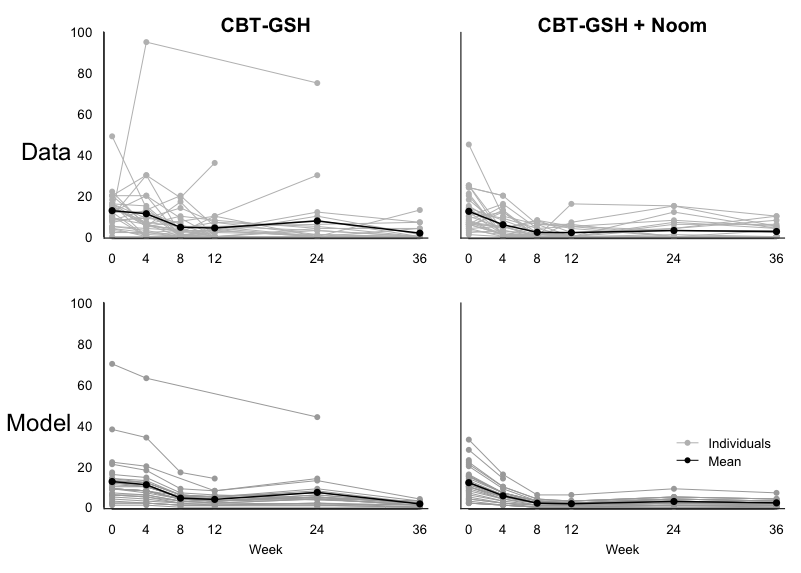
\includegraphics[width=\textwidth, height=\textheight, keepaspectratio]{ppc_sims.png}
\caption{\emph{Fig.3 (a) and (b) in the upper row show OBEs in each period for each individual in CBT - GSH and CBT-GSH + Noom respectively. Black dots represent mean estimate for each  period. Fig.3 (c) and (d) in the lower row show the simulated OBEs for each individual in CBT - GSH and CBT-GSH + Noom respectively. Black dots represent means from the simulated data for each period. The horizontal axis shows the week and the vertical axis shows the instances of OBE.}}
\end{center}
\end{figure}
%
Another way to check the fit of the model is by comparing simulated data directly against the raw data.  Figure 4 shows this for both treatment conditions.  Simulated data for the Noom condition appears to better track the raw data than simulated data for the no Noom condition.  This is unsurprising, since the no Noom condition tended to have more outliers, which we would not expect (or want) our model to pick up perfectly from such a small sample.  
%
\begin{figure}[H]
\begin{center}
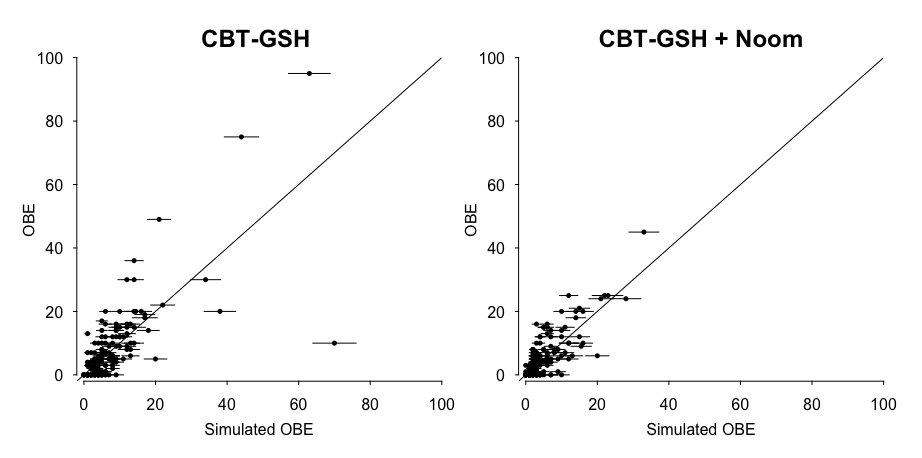
\includegraphics[width=\textwidth, height=\textheight, keepaspectratio]{obe_ppcs.png}
\caption{\emph{Fig. 4(a) and (b) show the predicted OBE vs. the actual OBE data for CBT - GSH and CBT- GSH + Noom respectively. The horizontal axis shows the simulated OBE and the vertical axis shows the actual OBE. The black dots are the points that represent this and the lines around them show 50\% intervals around the predictions. The upward sloping line is the 45 degree line.}}
\end{center}
\end{figure}
%
We conclude our model evaluations by mapping modeled density curves for each condition in each time period over the histograms in Figure 2.  Figure 5 shows that our model is able to broadly pick up on the patterns in the data over time and between treatment conditions. We see that the density curves clearly peak at lower values close to zero and have long tails, correctly capturing the pattern in the OBE data.

\begin{figure}[H]
\centering
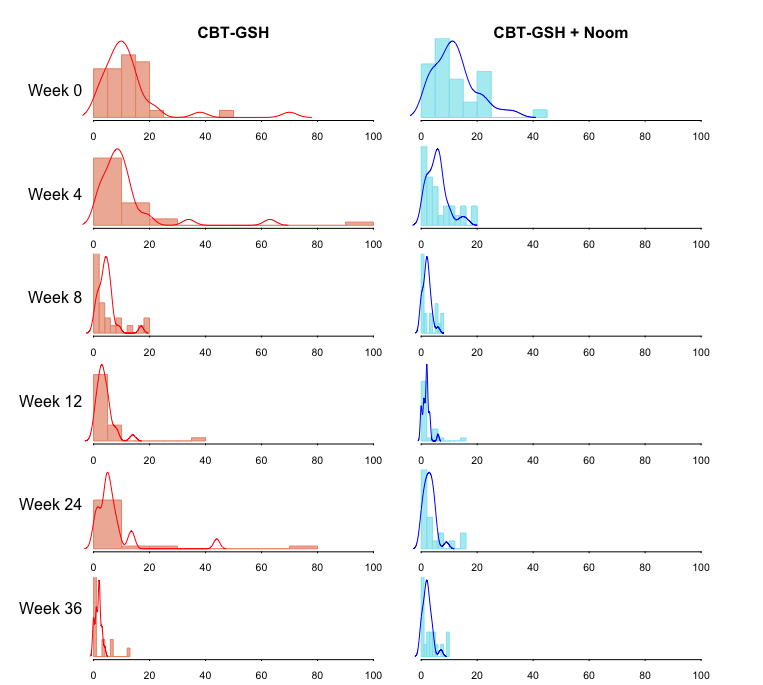
\includegraphics[width=\textwidth, height=\textheight, keepaspectratio]{ppc_hist_dens.png}
\caption{\emph{Histograms display the distribution of OBEs in each condition in each stage of the treatment. The orange and light blue histograms show the distribution of OBEs for the CBT-GSH and CBT-GSH  + Noom group respectively. The red and blue lines show the predicted density curves obtained from the simulations.}}
\end{figure}
Figure 6 displays the simulated OBE for both treatment groups (upper plot) and smoothed treatment effects (lower plot).  In each measurement period, simulated OBE are higher for the CBT - GSH condition than for the CBT - GSH + Noom condition, with some of the difference likely attributable to use of the Noom Monitor smartphone app.  This shows that the app has an effect on lowering episodes of binge eating.

\begin{figure}[H]
\begin{center}
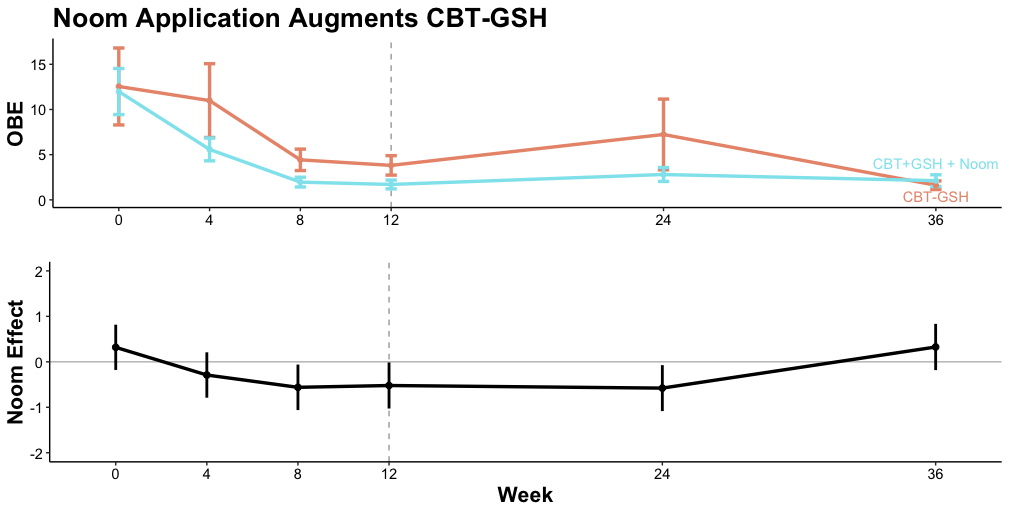
\includegraphics[width=\textwidth, height=\textheight, keepaspectratio]{noom_effect.png}
\caption{\emph{Fig. 6(a) the upper plot shows the simulated OBE in each time period. The CBT - GSH condition is in orange and the CBT - GSH + Noom condition is in orange. The bars around each point show the 95\% interval. Fig. 6(b) the lower plot shows the treatment effect for each period with the bars showing the 50\% interval. The horizontal axis shows the time period and the vertical axis for Fig.6 (a) shows the instances of OBE and for Fig.6 (b) shows the treatment effect of the Noom app.}}
\end{center}
\end{figure}

\section{Conclusion}
Bayesian Data Analysis is a powerful tool for incorporating data and prior information into simple and flexible models.  It is well-suited to analyze RCTs, where effects are small and data has complicated hierarchical structures.  In this paper, we have explained the steps of Bayesian Data Analysis and shown how they can be used to analyze an RCT that evaluates treatments for binge-eating disorder (BED) and bulimia nervosa (BN).  We model the impact of a smartphone app on binge eating behavior by fitting a hierarchical poisson model with individual level and time level effects, and time-varying treatment effects.  We find that the use of the smartphone app may cause a small reduction in Objective Bulimic Episodes in some stages of treatment.  We argue that Bayesian methodologies are well suited to analyzing RCTs on eating disorder behavior because they allow researchers to fit flexible models that explicitly include their assumptions and prior beliefs.


\newpage
\section{Appendix}
\subsection*{Example priors}
\begin{figure}[H]
\centering
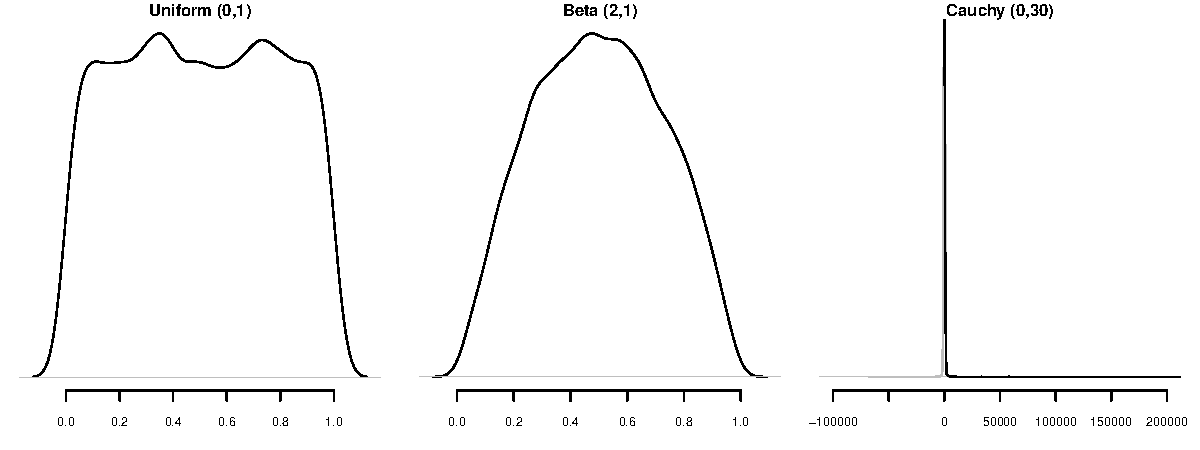
\includegraphics[width=\textwidth, height=\textheight, keepaspectratio]{prior_plot.pdf}
\caption{\emph{Fig. 7(a) shows a Uniform (0,1) distribution. Fig. 7(b) shows a Beta (2,1) distribution. Fig. 7(c) shows a Cauchy distribution, where the black line shows the positive half and the gray line shows the negative half.}}
\end{figure}
In Figure 7, we show some sample prior distributions. The Uniform (0,1) distribution (Fig. 7(a)) can be used when we know the quantity of interest is constrained to be between 0 and 1 but believe that all values between 0 and 1 are equally likely. If our quantity of interest is between 0 and 1 but unlikely to take extreme values we can use a Beta (2,1) (Fig. 7(b))  prior as shown.  Cauchy$^{+}$(0,30) is the half-Cauchy distribution with location 0 and scale 30 (Fig. 7(c)) . This is a good prior for variances because along with restricting the distribution to the positive real line it places most of the mass at 0 but allows for long smooth tails that the HMC algorithm can explore. 

\subsection*{Stan Model}
\begin{sexylisting}{Stan code}
data{\\ Declare data
  int N;
  int N_time;
  int N_ppl;
  int OBE[N];
  vector[N] tmt;
  int person_id[N];
  int time_id[N];
  int sex[N];
  int age[N];
  int black[N];
  int other_race[N];
  int hisp[N];
  int bn[N];
}
parameters{\\ Declare parameters for estimation
  real alpha[N_ppl];
  real mu_alpha;
  real<lower = 0> tau_alpha;
  real alpha_sex;
  real alpha_age;
  real alpha_black;
  real alpha_other;
  real alpha_hisp;
  real alpha_bn;
  real beta[N_time];
  real gamma[N_time];
  real mu_gamma;
  real<lower = 0> tau_gamma;
}
\end{sexylisting}
\begin{sexylisting}{Stan code contd.}
model{
  \\ Define likelihood
  for(i in 1:N) {
    OBE[i] ~ poisson_log(alpha[person_id[i]] + alpha_sex*sex[i] 
                         + alpha_black*black[i] 
                         + alpha_other*other_race[i]
                         + alpha_hisp*hisp[i] + alpha_bn*bn[i]
                         + beta[time_id[i]] + alpha_age*age[i]
                         + gamma[time_id[i]]*tmt[i]);
  }
  \\ Define priors
  alpha ~ normal(mu_alpha, tau_alpha);
  mu_alpha ~ normal(5, 2);
  tau_alpha ~ cauchy(0, 50);
  alpha_black ~ normal(0, 1);
  alpha_sex ~ normal(0, 1);
  alpha_other ~ normal(0, 1);
  alpha_hisp ~ normal(0, 1);
  alpha_bn ~ normal(0, 1);
  gamma ~ normal(mu_gamma, tau_gamma);
  mu_gamma ~ normal(0, 2);
  tau_gamma ~ cauchy(0, 30);
}
\end{sexylisting}
\begin{sexylisting}{Stan code contd.}
generated quantities{
  \\ Simulate data through the model
  real OBE_pred[N];
  for(i in 1:N) {
    OBE_pred[i] = poisson_log_rng(alpha[person_id[i]] 
                                  + alpha_sex*sex[i] 
                                  + alpha_black*black[i] 
                                  + alpha_other*other_race[i]
                                  + alpha_hisp*hisp[i] 
                                  + alpha_bn*bn[i]
                                  + beta[time_id[i]] 
                                  + alpha_age*age[i]
                                  + gamma[time_id[i]]*tmt[i]);
  }
}
\end{sexylisting}

\begin{thebibliography}{9}

\bibitem{A Conceptual Introduction to Hamiltonian Monte Carlo}
Betancourt M (2017).
\textit{``A Conceptual Introduction to Hamiltonian Monte Carlo"} 
arXiv:1701.02434 [stat.ME]

\bibitem{Calibrating Model-Based Inferences and Decisions}
Betancourt M (2018).
\textit{``Calibrating Model-Based Inferences and Decisions"} 
arXiv:1803.08393v1 [stat.ME]

\bibitem{Hierarchical Models for Causal Effects}
Feller, A and Gelman, A (2015) \textit{``Hierarchical Models for Causal Effects".}
Emerging Trends in the Social and Behavioral Sciences. Edited by Robert Scott and Stephen Kosslyn. ISBN 978-1-118-90077-2.

\bibitem{Visualization in Bayesian workflow}
Gabry J., Simpson D., Vehtari A., Betancourt M., Gelman A. (2018).
\textit{``Visualization in Bayesian workflow"} 
arXiv:1709.01449v4 [stat.ME]

\bibitem{Bayesian Data Analysis}
Gelman A, Carlin J.B, Stern H.S, Rubin D.B (2013).
\textit{``Bayesian Data Analysis"}
ISBN 0-412-03991-5, Chapman and Hall, New York

\bibitem{Prior distributions for variance parameters in hierarchical models(Comment on Article by Browne and Draper)}
Gelman A (2006).
\textit{``Prior distributions for variance parameters in hierarchical models(Comment on Article by Browne and Draper)"}
2006, International Society for Bayesian Analysis, Number 3, pp. 515 - 534.

\bibitem{Data Analysis Using Regression and Multilevel/Hierarchical Models}
Gelman A, Hill J (2007).
\textit{``Data Analysis Using Regression and Multilevel/Hierarchical Models"}
ISBN-13 978-0-521-68689-1, Published in the United States of America by Cambridge University Press, New York

\bibitem{Benefits and limitations of randomized controlled trials}
Gelman A (2017).
\textit{``Data Analysis Using Regression and Multilevel/Hierarchical Models"}

\bibitem{The benefits of using semi-continuous and continuous models to analyze binge eating data: A Monte Carlo investigation}
Grotzinger, A, Hildebrandt, T, and Yu, J. (2015). 
\textit{``The benefits of using semi-continuous and continuous models to analyze binge eating data: A Monte Carlo investigation."}
 Int J Eat Disord, 48(6), 746-758. doi:10.1002/eat.22351.
 
 \bibitem{Randomized controlled trial comparing smartphone assisted
versus traditional guided self-help for adults with binge eating}
Hildebrandt T, Michaelides A, Mackinnon D, Greif R, DeBar L, Sysko R (2017)
\textit{``Randomized controlled trial comparing smartphone assisted
versus traditional guided self-help for adults with binge eating"}
Int J Eat Disord. 2017 Nov;50(11):1313-1322. doi: 10.1002/eat.22781.

\bibitem{Stan}
Stan Development Team. 2016. 
\textit{RStan: the R interface to Stan}, Version 2.10.1.   
\texttt{http://mc-stan.org}

\bibitem{Stan}
Stan Development Team.
\textit{``Prior Choice Recommendations"}
\texttt{https://github.com/stan-dev/stan/wiki/Prior-Choice-Recommendations}

\bibitem{Exploratory Data Analysis}
Tukey J. (1977),
\textit{``Exploratory Data Analysis"}
ISBN-13: 978-0201076165.



\end{thebibliography}



\end{document}
